\newpage
\section{Diseño}
\subsection{Componentes cilíndricos bajo presión exterior}

El código indica, en el apartado \textbf{PG-27.2.2}, la expresión que debe utilizarse para determinar el espesor mínimo requerido para los caños (\textit{piping}), los domos (\textit{drums}), las envueltas (\textit{shells}) y los colectores (\textit{headers}).

\begin{equation}
     t = \frac{P \cdot D}{\num{2} \cdot S \cdot E + \num{2} \cdot y \cdot P} + C
     \label{eq:min_req_thickness_od}
\end{equation}

Aquí:
\begin{itemize}
     \item $\mathbf{D}$ es el diametro \underline{exterior} del componente cilíndrico. Una denominación alternativa es $\mathbf{OD}$ (\textit{outside diameter}). 
     
     El diámetro que debe utilizarse es el real, no el nominal. La unidad en que debe expresarse en la ecuación \ref{eq:min_req_thickness_od} es $\si{mm}$.
     
     Por ejemplo, para un caño de $\text{NPS}=\SI{10}{in}$ (\textit{nominal pipe size}), el diámetro nominal es $\text{DN}=\SI{250}{mm}$ mientras que el diámetro exterior es $\text{OD}=\SI{273.1}{mm}$. En este ejemplo, este último es el que debe utilizarse.

     Estos diámetros se establecen en el estándar \textbf{ASME B36.10M}, representando la M al estándar en el sistema métrico.

     \item $\mathbf{P}$ es la máxima presión admisible de trabajo (\textit{MAWP} o \textit{maximum allowable working pressure}). La presión que debe utilizarse, \underline{interna} en este caso, es la \underline{manométrica} o relativa al ambiente, ya que el esfuerzo sobre la pared del componente se genera a partir de la diferencia de fuerzas entre las originadas por la presión absoluta interior y la exterior (la atmosférica).
     
     Su definición se encuentra en el apartado \textbf{PG-21}. La unidad en que debe expresarse en la ecuación \ref{eq:min_req_thickness_od} es $\si{MPa(g)}$.   

     \item $\mathbf{S}$ es la máxima tensión admisible a la tempreatura de diseño del metal. En el apartado \textbf{PG-23} se indica que este valor máximo de tensión admisible puede encontrarse en la \textbf{sección II, parte D, subparte 1, tablas 1A y 1B} del \textbf{BPVC}.
     
     La unidad en que debe expresarse en la ecuación \ref{eq:min_req_thickness_od} es $\si{MPa}$.

     Más detalles pueden encontarse en el apartado \textbf{PG-27.4.2}.

     \item $\mathbf{E}$ es un valor adimensional denominado eficiencia. Más detalles pueden encontarse en el apartado \textbf{PG-27.4.1}.
     \item $\mathbf{y}$ es un coeficiente adimensional de temperatura. Más detalles pueden encontarse en el apartado \textbf{PG-27.4.6}.
     \item $\mathbf{C}$ es un ajuste o margen mínimo para que el componente tenga rigidez estructural (por ejemplo, que no sea sensible a posibles abolladuras por golpes en la manufactura, el transporte, en el caso de que algún operario se pare sobre este), y para tener en cuenta el roscado.
     
     Este margen se suma de manera directa, es un agregado al espesor requerido por el cálculo basado en la presión, el diámetro, la tensión admisible, la eficiencia y el coeficiente de temperatura.

     Más detalles pueden encontarse en el apartado \textbf{PG-27.4.3}.

\end{itemize}

En \textbf{PG-27.4.3} se establece que $C$ no incluyen ningún margen por una posible corrosión o erosión, por lo que este margen debe aplicarse en los casos en que sea necesario.

El código indica, en el mismo apartado, la expresión que debe utilizarse para determinar el espesor mínimo requerido a partir del radio interior (en lugar de determoinarlo respecto del diámetro exterior). Además, incluye las expresiones para determinar la presión interior máxima admisible de trabajo que soportan los componentes a partir de su espesor, tanto para el caso en que se conoce el diámetro exterior como el caso en que se conoce el radio interior.

\subsubsection{Relación con los esfuerzos teóricos}

La ecuación \ref{eq:min_req_thickness_od} puede relacionarse con la expresión de cálculo de la tensión en la dirección circunferencial $\sigma_{\theta}$ (\textit{hoop or circumferential stress}), a veces llamada tensión tangencial, para un cilindro de pared delgada sometido a una presión interior manométrica o relativa al ambiente:

\begin{equation}
     \sigma_{\theta}=\frac{P \cdot d}{\num{2} \cdot t}
     \label{eq:thin_wall_cylinder_int_pressure_01}
\end{equation}

Reagrupando,

\begin{equation}
     t=\frac{P \cdot d}{\num{2} \cdot \sigma_{\theta}}
     \label{eq:thin_wall_cylinder_int_pressure_02}
\end{equation}

La expresión \ref{eq:thin_wall_cylinder_int_pressure_01} se deriva de un equilibro estático de fuerzas entre la inducida por la presión interior (calculada a partir de la superficie proyectada) y la tensión que se genera en el espesor, por lo que aquí $d$ es el diámetro interior. Ver la figura \ref{im:thin_wall_cylinder_int_pressure_01}.

Un recipiente puede considerarse de pared delgada si el diámetro es, al menos, unas 20 veces el diámetro. Por lo tanto, para estos casos, la diferencia entre adoptar $d$ como el diámetro interior o exterior es despreciable.

\begin{figure}[ht]
     \centerline{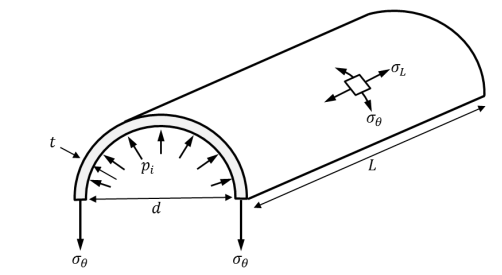
\includegraphics[scale=0.6]{thin_wall_cylinder_int_pressure_01.png}}
     \caption{\textit{Cilindro sometido a una presión interior.}}
     \label{im:thin_wall_cylinder_int_pressure_01}
\end{figure}

\begin{figure}[ht]
     \centerline{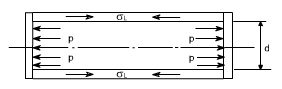
\includegraphics[scale=0.8]{thin_wall_cylinder_int_pressure_02.jpeg}}
     \caption{\textit{Cilindro sometido a una presión interior.}}
     \label{im:thin_wall_cylinder_int_pressure_02}
\end{figure}

La tensión en la dirección longitudinal $\sigma_L$ (\textit{longitudinal stress}), en el caso de que el cilindro tenga tapas, se calcula como

\begin{equation}
     \sigma_L=\frac{P \cdot d}{\num{4} \cdot t}
     \label{eq:thin_wall_cylinder_int_pressure_03}
\end{equation}

La expresión \ref{eq:thin_wall_cylinder_int_pressure_03} se deriva de un equilibro estático de fuerzas entre la inducida por la presión interior (calculada a partir de la superficie proyectada) y la tensión que se genera en el espesor, por lo que aquí $d$ es el diámetro interior. Ver la figura \ref{im:thin_wall_cylinder_int_pressure_02}.

Para un recipiente de pared delgada, la tensión en la dirección radial $\sigma_{r}$ (\textit{radial stress}) es mucho menor que las otras dos tensiones, y puede desestimarse. Por lo tanto, el sistema conforma un estado plano de tensiones perpendiculares entre sí, siendo $\sigma_{\theta}$ y $\sigma_L$ las tensiones principales de ese sistema.

\paragraph{Nota importante:} Si bien las ecuaciones \ref{eq:min_req_thickness_od} y \ref{eq:thin_wall_cylinder_int_pressure_01} están relacionadas, la que debe utilizarse al diseñar según el código es \ref{eq:min_req_thickness_od}, ya que esta contiene las características del material y sus propiedades, los efectos de la merma de resistencia del material por el efecto de la temperatura de diseño, la adopción de un coeficiente de seguridad, el debilitamientos en el caso de que el cilindro esté agujereado, el debilitamiento por las costuras de la soldadura, la adopción de un margen para una resistencia estructural propia ante golpes o abolladuras, el efecto del estado plano de tensiones, etc. 

\subsubsection{Ejemplo de cálculo}

Supongamos que se quiere dimensionar el espesor del domo de una caldera acuotubular. Consideremos una $\text{MAWP}=\SI{75}{bar(g)}$, una temperatura de diseño $T=\SI{290}{\celsius}$, que el diámetro exterior es $D=\SI{69,5}{in}=\SI{1765.3}{mm}$ que el material es SA-516 Gr. \num{70} y, únicamente para los fines de este ejemplo, que el domo no posee costuras de soldadura.

Determinando la eficiencia, el coeficiente de temperatura, la máxima tensión admisible a la temperatura de diseño del metal y considerando que no debe adicionarse el margen $C$, al reemplazar en \ref{eq:min_req_thickness_od}, resulta

\begin{gather*}
     t=\frac{\SI{7,5}{MPa(g)}\cdot\SI{1765,3}{mm}}{2\cdot\SI{137,6}{MPa}\cdot \num{1,0}+\num{2}\cdot \num{0,4}\cdot \SI{7,5}{MPa(g)}}\\
     \boxed{t=\SI{47,08}{mm}}
\end{gather*}


% Luego hacer la cuenta considerando la eficiencia.

\subsection{Material}

Acá quiero mostrar:

\begin{enumerate}
     \item La limitación de que el material tiene que estar en ASME II. PG-5.
     \item Para chapa (plate), veo PG-6.
     \item Para el ejemplo, dar las características del acero que utilizo. Sus valores de resistencia mecánica, las notas que lo rigen, el gráfico que hice, el valor de resistencia mecánica. ASME Parte 2
     \item Los apéndices no mandatorios del código ASME II sobre grafitización.
     \item La composición y el estándar ASTM que me rige. Esta en ASME II Parte A.
     \item Valor máximo de temperatura debe respetarse, a pesar de que esté listadas más temperaturas.
     \item En nota general de tabla IA me permite interpolar.
     \item STATEMENT OF POLICY ON INFORMATION PROVIDED IN THE STRESS TABLES. Acá figura esto del limite de temperatura, que no debe superarse. Ponerlo como nota al pie, o algo ais.
     \item Marcar que el código ya nos da los coeficientes de seguridad. Comparar la tensión que usamos contra el valor informado de fluecnia y de resistencia mecánica.
     \item Dar las características completas del material. Mencionar que está incorporado el estándar ASTM.
     \item El estándar ASTM está asociado a la forma en la que el material es comercializado (si es en chapa o barras, por ejemplo).
     \item Cada estándar tiene grados, que se relacionan con la resitencia.
     \item Creo que el código permite interpolar pero con la misma cantidad de decimales que el valor más chico, por lo que acá si no tengo decimales redondeo a 138. Hacer la cuenta con 138.
     \item 
\end{enumerate}

\begin{figure}[ht]
     \centerline{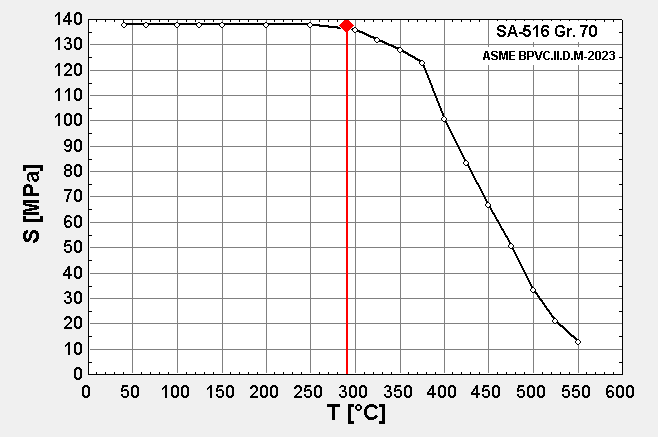
\includegraphics[scale=0.6]{mat_prop_example_01.png}}
     \caption{\textit{TBD.}}
     \label{im:mat_prop_example_01}
\end{figure}


\begin{table}[!ht]
     \centering
     \begin{tabular}{cc}
         \hline
         $\mathbf{T \left[\si{\celsius}\right]}$ & $\mathbf{S \left[\si{MPa}\right]}$ \\
         \hline
         $\num{40}$ & $\num{138}$ \\
         \hline
         $\num{65}$ & $\num{138}$ \\
         \hline
         $\num{100}$ & $\num{138}$ \\
         \hline
         $\num{125}$ & $\num{138}$ \\
         \hline
         $\num{150}$ & $\num{138}$ \\
         \hline
         $\num{200}$ & $\num{138}$ \\
         \hline
         $\num{250}$ & $\num{138}$ \\
         \hline
         $\num{300}$ & $\num{136}$ \\
         \hline
         $\num{325}$ & $\num{132}$ \\
         \hline
         $\num{350}$ & $\num{128}$ \\
         \hline
         $\num{375}$ & $\num{123}$ \\
         \hline
         $\num{400}$ & $\num{101}$ \\
         \hline
         $\num{425}$ & $\num{83.8}$ \\
         \hline
         $\num{450}$ & $\num{67.1}$ \\
         \hline
         $\num{475}$ & $\num{51.0}$ \\
         \hline
         $\num{500}$ & $\num{33.6}$ \\
         \hline
         $\num{525}$ & $\num{21.3}$ \\
         \hline
         $\num{550}$ & $\num{12.9}$ \\
         \hline
     \end{tabular}
     \caption{Poner qué es. De dónde la extraigo. Poner el limite de uso que figura, para usos según codigo asme I.}
     \label{tb:SA_516_70_S_value}
 \end{table}

\subsection{MAWP}

\subsection{Temperatura de diseño}

\subsection{Tensión admisible}

\subsection{Eficiencia}

\subsection{Coeficiente de temperatura}

\begin{enumerate}
     \item Acá voy a poner la temperatura de diseñp
\end{enumerate}










%PAGINA 20 tabla 1A

%linea 45

%resistencia mecanica minima 485 MPa
%fluencia minima 260 MPa
%G10 S1 T2
%Limite maximo de temperartura 454 C

%buscar si tengo algun calculo ferrer de estos
%tiene soldaduras longitudinales y cirfunferenciales

%cabezal de medida distinta a la envueltas
%Ver PG-6, que me admite este material
%considerando que domo va aislado, lo vamos a poner todo a temperatura de saturacion

%apendice de grafitizacion

%asme II non mandatorio A 201 y 202

%mencionar algo de la eficiencia de la soldadura. Medio que pasarlo por alto, la verdad.

%Lo mismo sobre los casquetes, para no marearme yo y no marear a los estudianbtes.

%Sí poner lo de la grafitizacion.






